\documentclass[12pt,a4paper]{ctexart}

\usepackage[UTF8]{ctex}
\usepackage{geometry}
\usepackage{graphicx}
\usepackage{xcolor}
\usepackage{tikz}
\usepackage{fontspec}
\usepackage{setspace}
\usepackage{enumitem}
\usepackage{booktabs}
\usepackage{array}
\usepackage{longtable}
\usepackage{hyperref}
\usepackage{fancyhdr}
\usepackage{titlesec}
\usepackage{multicol}
\usepackage{xurl}
\usepackage{tocloft}

\renewcommand{\cfttoctitlefont}{\hfill\bfseries\Large}
\renewcommand{\cftaftertoctitle}{\hfill}
\geometry{left=2.5cm,right=2.5cm,top=2.5cm,bottom=2.5cm}

\definecolor{black}{RGB}{0,0,0}
\definecolor{mainblue}{RGB}{0,82,147}
\definecolor{accentgold}{RGB}{180,140,60}
\definecolor{lightgray}{RGB}{245,245,245}
\definecolor{darkgray}{RGB}{80,80,80}
\definecolor{mainred}{RGB}{230,1,45}

\hypersetup{
    colorlinks=true,
    linkcolor=black,
    urlcolor=mainblue,
    citecolor=mainblue,
    pdfborder={0 0 0}
}

\pagestyle{fancy}
\fancyhf{}
\fancyhead[L]{\small\color{darkgray}\textbf{量子行业每周新闻洞察}}
\fancyhead[R]{\small\color{darkgray}\textbf{总第189期}}
\fancyfoot[C]{\thepage}
\renewcommand{\headrulewidth}{0.4pt}
\renewcommand{\footrulewidth}{0pt}

\titleformat{\section}
    {\Large\bfseries\color{mainred}}
    {\thesection、}{0em}{}
\titleformat{\subsection}
    {\large\bfseries\color{mainred}}
    {\thesubsection、}{0em}{}

\newcolumntype{L}[1]{>{\raggedright\arraybackslash}p{#1}}
\newcolumntype{C}[1]{>{\centering\arraybackslash}p{#1}}

\begin{document}

% ==================== 封面 ====================
\begin{titlepage}
\begin{tikzpicture}[remember picture,overlay]
    \fill[mainred] ([yshift=-0.5cm]current page.north west) rectangle ([yshift=-1.2cm]current page.north east);
    \fill[mainred] ([yshift=1.2cm]current page.south west) rectangle ([yshift=0.5cm]current page.south east);
\end{tikzpicture}

\vspace*{4cm}

\begin{center}
    {\fontsize{44}{52}\selectfont\bfseries\color{black} \textbf{量子行业每周新闻洞察}}

    \vspace{0.8cm}

    {\fontsize{16}{22}\selectfont\color{darkgray} 2026.07.19 — 2026.07.24 }
    {\fontsize{16}{22}\selectfont\color{darkgray} \textbf{WEEKLY NEWS}}

    \vspace{1.5cm}

    {\fontsize{20}{26}\selectfont\color{mainred}\textbf{（总第\textbf{ 189 }期）}}

    \vspace{4cm}

    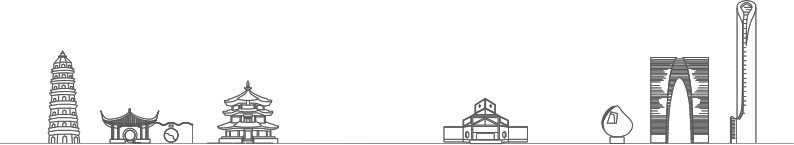
\includegraphics[width=\textwidth]{Cover_Suzhou.png}

    \vfill

    {\fontsize{12}{16}\selectfont\color{darkgray} 量子科技长三角产业创新中心\\编制：战略情报与成果专利室、产业发展部（理事会办公室）}
\end{center}
\end{titlepage}

% ==================== 目录 ====================
\pagenumbering{roman}
\newpage
\tableofcontents

\newpage

% ==================== 摘要 ====================
\pagenumbering{arabic}
\setcounter{page}{1}
\begin{center}
{\Large\bfseries\color{mainred} 摘\hspace{2em}要}
\end{center}
\addcontentsline{toc}{section}{摘要}


\textbf{ 宏观态势：}

本周该领域保持活跃态势。


\textbf{ 科技前沿：}

本周该领域保持活跃态势。


\textbf{ 产品动态：}

本周该领域保持活跃态势。


\textbf{ 企业资讯：}

本周该领域保持活跃态势。


\textbf{ 资本运作：}

本周该领域保持活跃态势。




\textbf{ 专利动态：}

本周专利动态涵盖低温环境系统、超导量子测控技术、量子软件与算法、量子科技长三角产业创新中心共4个板块、19条专利。




% ==================== 会议列表 ====================
{
    \newpage
    \section*{ 8月量子科技行业国内、国际会议}
    \addcontentsline{toc}{section}{ 8月量子科技行业国内、国际会议}
    \scriptsize
    \begin{longtable}{C{0.8cm}L{2.5cm}L{3cm}L{7cm}}
        \toprule[1.5pt]
        \textbf{序号} & \textbf{日期} & \textbf{地点} & \textbf{会议名称} \\
        \midrule
        \endfirsthead
        \toprule
        \textbf{序号} & \textbf{日期} & \textbf{地点} & \textbf{会议名称} \\
        \midrule
        \endhead
        \bottomrule
        \endfoot
        
        1 & 8月3日-5日 & 博尔德及线上, 美国 & 天气与气候应用的量子计算与传感研讨会 \\
        \midrule[0.05pt]
        
        2 & 8月3日-14日 & 贝纳斯克, 西班牙 & 容错量子技术研讨会 \\
        \midrule[0.05pt]
        
        3 & 8月7日-9日 & 杭州, 中国 & 第2届量子计算与通信技术国际会议（ICQCT 2026） \\
        \midrule[0.05pt]
        
        4 & 8月10日-14日 & 纳塔尔, 巴西 & 量子热力学会议2026（QTD 2026） \\
        \midrule[0.05pt]
        
        5 & 8月10日-14日 & 阿姆斯特丹, 荷兰 & QSim2026 \\
        \midrule[0.05pt]
        
        6 & 8月14日-16日 & 印第安纳波利斯, 美国 & 量子AI与自然语言处理2026会议（QNLPAI 2026） \\
        \midrule[0.05pt]
        
        7 & 8月16日-21日 & 巴德洪内夫, 德国 & 量子机器学习暑期学校（Bad Honnef物理学校） \\
        \midrule[0.05pt]
        
        8 & 8月16日-22日 & 贝纳斯克, 西班牙 & 悬浮系统量子工程研讨会 \\
        \midrule[0.05pt]
        
        9 & 8月17日-21日 & 多伦多, 加拿大 & 第11届量子信息与量子控制会议（CQIQC-XI） \\
        \midrule[0.05pt]
        
        10 & 8月17日-21日 & 阿姆斯特丹, 荷兰 & 第23届量子物理与逻辑国际会议（QPL 2026） \\
        \midrule[0.05pt]
        
        11 & 8月24日-28日 & 渥太华, 加拿大 & QCrypt 2026 \\
        \midrule[0.05pt]
        
        12 & 8月24日-28日 & 大田, 韩国 & 第26届亚洲量子信息科学会议 (AQIS) \\
        \midrule[0.05pt]
        
        13 & 8月24日-28日 & 维也纳, 奥地利 & 第9届青年量子信息科学家国际会议 (YQIS) \\
        \midrule[0.05pt]
        
        14 & 8月25日-28日 & 哥德堡, 瑞典 & 超导量子比特与算法 2026 (SQA) \\
        \midrule[0.05pt]
        
        15 & 8月30日-9月1日 & 布雷钦, 英国 & 量子ARC写作静修 \\
        \midrule[0.05pt]
        
        16 & 8月31日-9月3日 & 仁川, 韩国 & 硅量子电子学研讨会 2026 (SiQEW) \\
        \midrule[0.05pt]
        
        17 & 8月31日-9月3日 & 泰恩河畔纽卡斯尔, 英国 & Photon 2026 \\
        \midrule[0.05pt]
        
        18 & 8月31日-9月4日 & 瓦莱塔, 马耳他 & Qalypso 2026暑期学校—量子优化技术与计算物理 \\
        \midrule[0.05pt]
        
        19 & 8月31日-9月4日 & 舍布鲁克, 加拿大 & 量子计算、通信与密码学理论 2026 (TQC) \\
        \midrule[0.05pt]
        
        20 & 8月31日-9月10日 & 格但斯克, 波兰 & Q-Camp: 量子暑期学校 2026 \\
        \midrule[0.05pt]
        
    \end{longtable}
}




% ==================== 宏观态势 ====================
\newpage
\section{宏观态势}
\vspace{-0.5em}
\noindent\rule{\linewidth}{1.5pt}

\subsection{ IberianQCI项目近期启动 将推进西葡跨境量子通信基础设施建设 }

2026年07月23日消息，伊比利亚量子通信基础设施（IberianQCI）项目已于2026年5月正式启动，标志着欧洲量子通信基础设施（EuroQCI）计划取得进一步进展。该项目由西班牙Indra Space公司协调，汇集葡萄牙和西班牙两国领先科研与产业伙伴，旨在通过地面与空间相结合的方式，互联西班牙EuroQCI Spain和葡萄牙PTQCI国家量子通信网络。项目周期超过三年，主要推进两大方向：一是利用量子密钥分发（QKD）技术在葡西北部边境建立跨境量子通信链路；二是在葡萄牙部署1座、西班牙部署3座光学地面终端（OGT），实现EuroQCI空间段与地面网络的无缝互联。其中位于巴塞罗那的OGT由西班牙光子科学研究所（ICFO）牵头安装与调试。

\noindent\textbf{报道链接：}\url{https://www.icfo.eu/news/2694/start-of-iberianqci-the-quantum-communications-infrastructure-of-the-euroqci-program-for-spain-and-portugal/880/}

\subsection{ 新加坡国防部联手IBM，探索量子计算在军事任务优化中的应用潜力 }

2026年07月24日消息，新加坡国防部近日宣布，新加坡武装部队（SAF）数字与情报部队（DIS）和国防科技局（DSTA）已与IBM达成合作，共同探索量子计算在国防任务规划中的应用潜力，重点面向复杂任务规划和后勤优化等场景。根据合作计划，DIS和DSTA工程师将与IBM专家联合开发并评估量子优化算法，并通过IBM云端量子计算平台开展实验验证和性能测试，同时积累量子算法开发与编程框架等本土技术能力。

\noindent\textbf{报道链接：}\url{https://www.janes.com/defence-intelligence-insights/defence-news/defence/singapore-ibm-partner-on-defence-quantum-computing}

\subsection{ 荷兰启动450万欧元量子技术研究资助计划 聚焦便携式纠缠与PQC两大主题 }

2026年07月23日消息，荷兰科学研究组织（NWO）近日开放一项总额约450万欧元的“量子时代的安全与韧性”资助申请，面向荷兰科研人员开展量子领域前沿探索。该计划设立两个研究方向：方向一为量子网络中的便携式纠缠，旨在探索纠缠“可携带化”的途径，并能长时间保存在量子存储器中；方向二为后量子密码学，旨在提升现有及新型加密算法、方案与协议的安全认知与可信度，要求这些技术能抵御量子攻击，同时可在传统ICT系统上部署。每个项目在方向一可申请100万至150万欧元补贴，方向二最高为38.5万欧元，每个方向排名前两位的申请将获得资助。

\noindent\textbf{报道链接：}\url{https://www.nwo.nl/en/news/call-open-around-eu45m-available-for-fundamental-research-on-quantum-technology}

\subsection{ 以色列创新局启动1亿新谢克尔国家量子计算研发基础设施计划 }

2026年07月23日消息，以色列创新局近日发布一项新的项目招标，计划投入1亿新谢克尔（约合2700万美元）建立国家级量子计算研发基础设施。该基础设施将集成至少三种不同的量子处理技术，将作为一个全国性量子计算评估、集成与应用中心，向以色列产业界和学术界开放。基础设施将覆盖量子计算全栈研发服务，涵盖硬件与量子比特、控制与测量系统、纠错、软件算法到用户界面及应用开发。根据要求，该设施须在获批后18个月内全面建成，并在前12个月内开始向用户提供包括硬件访问、云服务和算法评估在内的研发服务。

\noindent\textbf{报道链接：}\url{https://innovationisrael.org.il/en/press\_release/quantum-infrastructure/}

\subsection{ 大阪大学与G-QuAT被选中参与日本量子计算产业化人才培养项目 }

2026年07月23日消息，日本新能源产业技术综合开发机构（NEDO）近日选定大阪大学与日本产业技术综合研究所（AIST）旗下G-QuAT中心作为其量子计算产业化人才培养项目的执行机构。该项目计划执行期为2026至2028年度，合同金额约29.99亿日元（约合人民币1.25亿元）。根据项目安排，大阪大学量子信息科学方向的研究生将可利用AIST的尖端设施开展博士阶段前沿研究，构建产业界所需的高技能专业人才培养体系，以缓解日本量子计算专业人才短缺，并增强其量子产业竞争力。

\noindent\textbf{报道链接：}\url{https://www.osaka-u.ac.jp/en/news/topics/2026/07/17002}

\subsection{ 美国白宫承诺超50亿美元扩大“创世纪计划”，量子技术列为核心方向 }

2026年07月23日消息，美国白宫昨日宣布，将投入超50亿美元扩展面向“AI赋能科学”的国家级“创世纪任务”，并启动覆盖医疗、能源、基础设施、制造和前沿科研的国家科技挑战。该计划由超15个以上联邦机构参与，依托美国能源部建设的科学与安全平台，向研究人员开放数据、算力、AI工具及科研设施。首批共有278个项目入选。量子领域方面，能源部与国防部将利用AI加速量子计算、量子传感和量子通信研发，包括推动建设具备科学实用价值的容错量子计算机，以及将量子传感器用于定位、导航和授时等实际场景。

\noindent\textbf{报道链接：}\url{https://www.hpcwire.com/off-the-wire/white-house-commits-more-than-5b-to-expand-genesis-mission/}

\subsection{ 越南即将举办首届国际量子计算黑客松竞赛决赛 }

2026年07月21日消息，越南即将举办首届国际量子计算黑客松竞赛“QC4SG 2026”决赛，这是该国首次举办国际性量子计算黑客松活动，也是东南亚第二个同类赛事。赛事由越南国家创新中心、越南量子技术创新网络VNQuantum等机构共同推动，旨在发掘量子领域创新项目和青年人才，促进量子技术成果转化，并进一步加强越南与国际量子科技生态的合作，加快构建区域量子创新与产业发展能力。

\noindent\textbf{报道链接：}\url{https://vietnamnet.vn/en/vietnam-hosts-first-international-quantum-computing-hackathon-2537546.html}

\subsection{ 澳大利亚信号局发布量子安全指南，五步法评估供应商量子就绪性情况 }

2026年07月21日消息，澳大利亚信号局（ASD）近日发布一份实用指南，旨在帮助机构评估第三方供应商的量子安全准备情况。该指南依据ASD的LATICE框架，将评估划分为五个阶段：定位并盘点密码依赖、评估单个系统风险、筛选并确定迁移优先级、实施符合国际标准的后量子密码算法，以及与供应商沟通并开展利益相关方教育。该指南强调，企业和政府普遍依赖云平台、托管服务及外部工具，若供应商迁移缓慢或缺乏系统可见性，相关数据仍可能面临风险。

\noindent\textbf{报道链接：}\url{https://pqshield.com/australia-issues-guidance-on-evaluating-third-party-quantum-readiness/}

\subsection{ 全球量子论坛将于近日在芝加哥开幕，聚焦利用量子技术解决重大社会挑战 }

2026年07月21日消息，第二届全球量子论坛（GQF）以“应对重大挑战”为主题将于7月22日至23日在芝加哥举行，由P33与伊利诺伊州经济发展公司（Illinois EDC）联合主办。据悉，与专注技术层面的量子会议不同，该论坛旨在汇聚国际量子企业、研究人员、科学家、投资者及政策制定者，探讨量子技术如何应对网络安全强化、能源系统现代化及加速医学突破等社会最复杂问题。

\noindent\textbf{报道链接：}\url{https://www.prnewswire.com/news-releases/global-leaders-fortune-500-ceos-and-tech-visionaries-convene-in-chicago-for-second-annual-global-quantum-forum-302829970.html}


% ==================== 科技前沿 ====================
\newpage
\section{科技前沿}
\vspace{-0.5em}
\noindent\rule{\linewidth}{1.5pt}

\subsection{ 密歇根大学研发新型半导体器件，可仅用激光控制电子流动，无需电源 }

2026年07月23日消息，美国密歇根大学的一个研究团队近日打造出一种新型半导体器件，仅凭激光即可控制电子在半导体中的流动，无需任何电源。该团队在纳米制造设施中制造了这一器件，它有潜力发展成为一种可测量各种光特性的仪器。利用该器件，研究人员证明，通过使用两种不同颜色的光，可以诱导电子在半导体中有序流动，而通过旋转两种光场的偏振方向，还能操控电流方向。相关研究成果已于日前发表在《物理评论快报》上。

\noindent\textbf{报道链接：}\url{https://www.eurekalert.org/news-releases/1136862}

\subsection{ IonQ与QuantumBasel合作探索量子硬件在混合AI工作负载中的能效潜力 }

2026年07月23日消息，IonQ与QuantumBasel的研究团队近日发布一项联合研究成果，表明在特定混合量子-经典AI工作负载中，量子硬件有望在能源效率方面超越经典方案。团队在IonQ的36量子比特Forte Enterprise囚禁离子量子计算机上，直接测量了其执行量子电路微调基础AI模型时的实际功耗。数据显示，量子处理器能耗随量子比特数呈近似线性增长，而经典GPU模拟相同电路的能耗呈指数增长。基于实测数据，研究预测约在34量子比特处实现能耗盈亏平衡。在情感分析基准测试中，经误差缓解后的量子模型准确率达91.2\%，超过逻辑回归和支持向量机等传统方法。该研究已提交至IEEE量子周会议，并发表于arXiv预印本平台。

\noindent\textbf{报道链接：}\url{https://thequantuminsider.com/2026/07/21/ionq-quantumbasel-study-suggests-hybrid-ai-workloads-could-gain-energy-advantages-from-quantum-hardware-as-systems-scale/}

\subsection{ 俄罗斯研究团队首次用光学方法观测二维材料中的维格纳晶体 }

2026年07月23日消息，俄罗斯量子中心、圣光机大学和莫斯科物理技术学院的研究人员近日首次证明，可通过光学方式观测超薄材料中电子的集体行为。该团队在约1纳米厚的单层二硒化钨中捕捉到维格纳晶体的特征，即低温电子由无序运动转变为规则排列，并首次在无需强磁场的条件下，通过材料对光的响应识别这一状态。该方法省去了复杂电接触系统和强磁场装置，有望简化超导、特殊磁性及新型电子态等研究。相关研究成果已于近日发表在《物理评论B》期刊。

\noindent\textbf{报道链接：}\url{https://www1.ru/en/news/2026/07/21/materialy-budushhego-vpervye-udalos-uvidet-s-pomoshhiu-sveta-novoe-otkrytie-rossiiskix-ucenyx.html}

\subsection{ QuantX Labs研发的光学频率梳已在轨完成调试并投入运行 }

2026年07月21日消息，澳大利亚量子技术公司QuantX Labs今日宣布，其研发的光学频率梳已在轨成功完成调试并投入运行。这标志着澳大利亚在航天与量子技术领域取得一项重大里程碑，并首次在轨展示了世界级量子计时能力。该任务得到澳大利亚航天局“月球到火星示范计划”的支持，是QuantX Labs旗下KAIROS项目的关键组成部分，该项目旨在开发面向空间应用的下一代精密计时技术。这一进展表明，其研制的光学频率梳不仅经受住了发射与部署的考验，而且在严苛太空环境下能按设计正常工作，这也向在轨部署全球首台光学原子钟迈出了重要一步。

\noindent\textbf{报道链接：}\url{https://quantxlabs.com/news/quant-x-labs-announces-successful-in-orbit-commissioning-of-worlds-first-optical-frequency-comb/}

\subsection{ 德国科学家首次直接观测到磁子的自发宏观相干性 }

2026年07月21日消息，德国凯泽斯劳滕-兰道大学的一个研究团队最近取得了一项关键的实验突破：首次直接观测到了磁子（磁性材料中的量子化激发）的自发宏观相干性。该实验证实了磁子玻色-爱因斯坦凝聚（BEC）理论的核心预言。研究人员利用高精度相位分辨微波光谱学，在重复实验中直接观测到了相干性的涌现以及冷凝液相的随机播种过程。该成果首次为磁子BEC的这一标志性特征提供了实验证据，有望为信号处理、传感技术及信息处理开辟新路径。相关研究已于日前发表在《自然物理学》期刊上。

\noindent\textbf{报道链接：}\url{https://phys.org/news/2026-07-spontaneous-magnon-coherence-room-temperature.html}

\subsection{ SLAC国家加速器实验室与Q-NEXT的研究人员正开发基于量子点的量子比特 }

2026年07月22日消息，美国能源部SLAC国家加速器实验室与Q-NEXT量子信息科学研究中心的研究人员正在开发基于量子点的量子比特。目前，该团队正围绕量子点量子比特的材料、器件和系统架构开展研究，重点解决大规模集成过程中噪声控制、器件互连、运行温度及软件控制等关键问题，以提升量子比特的稳定性和可扩展性。相比其他量子比特技术路线，量子点量子比特可采用成熟半导体工艺实现批量制造，有望在单块芯片上集成数百万甚至数十亿个量子比特，为构建大规模量子计算机提供基础。

\noindent\textbf{报道链接：}\url{https://www.newswise.com/doescience/containing-multitudes-slac-scientist-collaborates-to-create-scalable-qubits/?article\_id=851117}

\subsection{ 大阪大学与日本产业技术综合研究所将共建量子计算高端人才培养基地 }

2026年07月22日消息，大阪大学与日本产业技术综合研究所（AIST）日前宣布，双方联合申报的量子计算产业化人才培养项目获日本新能源产业技术综合开发机构（NEDO）选中，成为现阶段唯一入选项目，实施期计划为2026至2028年度。项目将以大阪大学“量子信息科学学位项目”为基础，由量子信息与量子生命研究中心（QIQB）和量子与AI融合技术业务开发全球研究中心（G-QuAT）合作，为量子信息科学博士生开放先进设备和研究环境，支持其开展前沿研究，并建立连接高校科研与产业需求的人才培养机制。项目旨在培养具备量子计算研发及产业化能力的高端专业人才，增强日本量子产业的竞争力与持续发展能力。

\noindent\textbf{报道链接：}\url{https://qiqb.osaka-u.ac.jp/newstopics/pr20260717}

\subsection{ 东京大学科学家利用反铁磁体成功实现无需焦耳热辅助的磁状态电学切换 }

2026年07月22日消息，东京大学的研究人员最近在反铁磁体中成功展示了无需焦耳热辅助的磁状态电学切换机制。该研究表明，通过优化Mn3Sn薄膜器件的厚度以有效散去产生的热量，可以实现一种不依赖热生成与冷却过程、而是直接利用反铁磁体皮秒级本征高速磁动力学自旋轨道矩切换机制。当薄膜厚度减薄以减少热效应时，磁切换从由热辅助控制的机制转变为自旋电流直接调控反铁磁序的内源机制。这种内源机制支持更短的电流脉冲操作，有望显著降低能耗。相关成果已于日前发表在《自然·通讯》上，为利用反铁磁体超快磁动力学实现新型非易失性存储技术奠定了重要基础。

\noindent\textbf{报道链接：}\url{https://www.s.u-tokyo.ac.jp/en/press/11188/}

\subsection{ 谷歌利用强化学习实现了在量子计算运行中进行持续校准 }

2026年07月21日消息，由谷歌领导的一个研究团队在Willow超导量子处理器上验证了一种基于强化学习的持续校准方法，使量子计算机可在执行量子纠错的同时，根据自身错误数据动态调整运行参数。该系统利用纠错过程中产生的错误检测事件作为反馈，持续优化微波脉冲幅度、频率、耦合强度等大量控制参数，无需中断计算进行周期性校准。实验显示，该方法在传统校准和专家调优基础上进一步将逻辑错误率降低约20\%；在人为引入硬件漂移的条件下，配合解码器参数调整可将逻辑错误率降低31\%，稳定性提升3.5倍。该研究为未来容错量子计算机长时间自主运行提供了潜在技术路径，相关成果已发表于近期的《自然》杂志。

\noindent\textbf{报道链接：}\url{https://thequantuminsider.com/2026/07/10/google-study-shows-quantum-computer-can-learn-from-its-own-errors-while-it-computes/}

\subsection{ Quantinuum联合多所高校成功实现基于非阿贝尔任意子的通用量子门 }

2026年07月21日消息，Quantinuum与加州理工学院、芝加哥大学及哈佛大学组成的研究团队，在该公司的System Model H2离子阱量子计算机上制备出一种罕见的拓扑有序物质态，并利用由此产生的非阿贝尔任意子执行了受保护的通用量子门和测量。研究人员通过“编织”任意子实现量子操作，使量子信息分布于整个系统，从而增强其对噪声和局部误差的抵抗能力。该方法为容错量子计算提供了不同于传统纠错方案的技术路径，有望减少对资源开销较大的魔法态蒸馏流程的依赖，降低未来通用容错量子计算所需的物理量子比特数量和运行时间。相关成果发表于近期的《自然》期刊。

\noindent\textbf{报道链接：}\url{https://www.quantinuum.com/blog/a-new-state-in-quantum-computing}

\subsection{ 新研究发现：在适合条件下量子系统可通过耗散实现纠缠 }

2026年07月21日消息，美国伊利诺伊大学厄巴纳-香槟分校与芝加哥大学的研究人员合作，通过一项实验验证了一项理论预测：在外部驱动下，量子系统可通过耗散（即能量和信息不可避免地泄漏到环境中）实现纠缠。传统上，耗散被视为量子技术的敌人，但该团队开发出一种名为“合成压缩”的新技术，利用一对超导量子比特，在实验室中成功再现了这一现象。研究人员认为，这一成果有望作为现有纠缠生成方法的更稳健、可靠的替代方案，为量子技术的应用提供新的路径。

\noindent\textbf{报道链接：}\url{https://www.newswise.com/articles/entanglement-over-large-separations-because-of-not-despite-dissipation}

\subsection{ 中国科大新研究表明：量子隐形传态在远距离量子通信中性能要优于光子直接传输 }

2026年07月20日消息，中国科学技术大学的研究人员最近证明，在远距离量子通信中，量子隐形传态比直接传输光子更具优势，能帮助克服光子损失问题。该研究团队开发了一种全光学方案，可远程制备高质量纠缠光子对并实现量子隐形传态。在该研究中，他们让量子隐形传态与直接光子传输进行“同台竞技”，结果发现，即使直接传输光子使用了最优量子克隆技术进行增强，量子隐形传态的传输效率仍是它的近三倍。这一结果证明了该隐形传态方案具有无条件的性能优势，有望为构建长距离、低损耗的量子通信网络提供新路径。相关研究成果已于日前发表在《自然物理学》上。

\noindent\textbf{报道链接：}\url{https://phys.org/news/2026-07-quantum-teleportation-photon-loss-distance.html}

\subsection{ 以色列科研团队成功实现按需生成抗噪的高质量偏振纠缠光子对 }

2026年07月20日消息，以色列量子计算公司Quantum Source近日宣布，它与以色列国防研究与发展局（DDR\&D）合作实现了高质量偏振纠缠光子对的可控按需生成，且光子对处于鲁棒的量子单态。团队还展示了该状态的卓越抗噪能力：在标准光纤中传输超过一公里，且传输条件任意、持续变化的情况下，其纠缠保真度未出现可测量的退化，而且整个过程未使用任何主动偏振稳定、反馈或信道校准。该公司表示，这一技术有望支持未来的量子通信网络、量子中继器、分布式量子计算和量子互联网基础设施。

\noindent\textbf{报道链接：}\url{https://thequantuminsider.com/2026/07/16/quantum-source-robust-entangled-photon-source-quantum-networks/}


% ==================== 产品动态 ====================
\newpage
\section{产品动态}
\vspace{-0.5em}
\noindent\rule{\linewidth}{1.5pt}

\subsection{ IBM将向美国“创世任务”提供5000万美元量子算力 并有量子应用开发项目被选中 }

2026年07月24日消息，IBM昨日宣布，将为美国能源部“创世任务”提供最高价值5000万美元的全球领先公用事业级量子计算资源，并被选中牵头一项利用AI加速量子应用发现的研究项目。相关算力将基于156量子比特Heron和120量子比特Nighthawk处理器，面向美国能源部国家实验室及其合作伙伴开放。IBM表，目前其拥有15台投入运行的量子计算机，平均正常运行时间超过97\%，可全天候为超过25万名用户提供服务。最新的Nighthawk系统支持120个可编程量子比特，每秒可执行超过5000次QuOps，吞吐量高达每秒10万个量子电路。

\noindent\textbf{报道链接：}\url{https://research.ibm.com/blog/ibm-us-genesis-mission-quantum-ai}

\subsection{ Infleqtion将于2027年向伊利诺伊IQMP园区交付中性原子容错量子计算机 }

2026年07月24日消息，Infleqtion日前宣布，将于2027年向伊利诺伊量子与微电子园区（IQMP）交付其基于中性原子技术的容错量子计算机。该公司还在芝加哥新设量子创新中心，以扩大量子计算应用研发，并持续增加伊利诺伊州的劳动力与投资。据了解，Infleqtion的Sqale系统是一款全栈量子计算平台，专为容错性能而设计，集成了英伟达NVQLink技术，可实现量子处理器与GPU加速计算之间的低延迟耦合。该系统旨在实现超过50个逻辑量子比特，并向项目100个逻辑量子比特的目标推进，其架构支持扩展至1000个以上物理量子比特。

\noindent\textbf{报道链接：}\url{https://infleqtion.com/infleqtion-to-deploy-fault-tolerant-neutral-atom-quantum-computer-in-illinois/}

\subsection{ Qedma的纠错软件已集成至Quantinuum平台，助力量子电路处理更复杂任务 }

2026年07月24日消息，Qedma日前宣布与Quantinuum平台完成技术集成，用户现可在后者的量子计算硬件上使用Qedma先进的纠错方案。据悉，Qedma的量子错误抑制与纠错（QESEM）软件能够在诸多应用中提升计算精度，支持更大规模和更复杂的量子电路。在典型工作流程中，QESEM可有效缓解量子计算输出的错误，帮助研究人员应对日益复杂的计算任务，以追求商业与科学上的优势。

\noindent\textbf{报道链接：}\url{https://www.prnewswire.com/news-releases/qedma-integrates-its-advanced-error-mitigation-software-with-quantinuums-quantum-computing-platform-302833149.html}

\subsection{ QURECA携手SpinFlex推spinEDU量子教育套件，强化实践型量子学习资源 }

2026年07月23日消息，QURECA近日宣布与SpinFlex Instruments达成合作，将后者开发的spinEDU教育套件纳入其量子教育资源体系，以扩展面向学生、教育工作者和专业培训提供商的实践型学习工具。spinEDU以固态钻石自旋量子比特的真实实验为核心，旨在帮助学习者通过实验操作理解量子技术相关概念。此次合作将进一步丰富QURECA在量子计算教育领域的培训内容，将推动量子知识从理论教学向动手实践延伸。

\noindent\textbf{报道链接：}\url{https://www.qureca.com/quantum-education-resources-qureca-partners-with-spinflex-to-expand-hands-on-learning-with-spinedu/}

\subsection{ 日本首台国产光量子计算机MoQuren已部署在AIST旗下研究中心 }

2026年07月22日消息，日本OptQC公司与日本产业技术综合研究所（AIST）今日宣布，OptQC的首台光量子计算机“MoQuren”已在AIST的全球量子-AI 技术商业全球研发中心（G-QuAT）成功安装并投入运行。这是全球首次将日本制造的、面向未来商业化的光量子计算机部署在实用研究开发环境中。MoQuren采用室温运行设计，具备出色的可扩展性，其运行旨在通过将OptQC的光量子技术集成至AIST的ABCI-Q平台，构建一个能够解决复杂现实问题的计算系统。

\noindent\textbf{报道链接：}\url{https://www.aist.go.jp/aist\_e/news/au20260722.html}

\subsection{ Interlune利用其冷捕获技术成功从A级氦中生产出纯度达99\%的氦-3 }

2026年07月22日消息，太空基础设施与资源公司Interlune日前宣布，其“冷捕获”技术已成功从A级氦中生产出纯度达99\%的氦-3。该技术若大规模部署，有望将美国目前用于量子计算的这一关键同位素供应量提升两倍。此前，Interlune于2025年初展示了该技术，并于同年11月获得AFWERX小企业创新研究（SBIR）直接进入第二阶段合同，旨在将该技术规模化至工业级氦气生产。

\noindent\textbf{报道链接：}\url{https://www.prnewswire.com/news-releases/interlune-produces-pure-helium-3-from-domestic-helium-using-novel-cryogenic-technology-302829735.html}

\subsection{ SAXON Q推出128量子比特和512量子比特的商用氮空位色心量子计算系统 }

2026年07月22日消息，德国金刚石氮空位（NV）色心量子计算先驱SAXON Q昨日宣布，其128量子比特SXQ128和512量子比特SXQ512系统已正式商用，这是首批超过10量子比特的金刚石NV色心量子计算机。两款系统均在室温下运行，无需低温冷却、真空设备或特殊设施。该系统采用半导体兼容制造工艺，可装入标准服务器机架、接入标准电源，无需传统量子计算所需的重新校准周期或环境控制。SAXON Q平台还是唯一支持跨多个量子处理核心同时协调计算的商用NV色心量子计算系统，通过其专有多核量子操作系统，SXQ128每个核心能提供8个完全纠缠的量子比特，SXQ512则每个核心则为16个。

\noindent\textbf{报道链接：}\url{https://www.hpcwire.com/off-the-wire/saxon-q-brings-room-temperature-diamond-quantum-computing-to-commercial-market/}

\subsection{ Two Hands公司正推进量子模拟软件平台EntangleX的研发 }

2026年07月22日消息，Two Hands公司昨日公布了其量子模拟软件平台EntangleX的最新研发进展。该平台旨在通过传统GPU基础设施，降低量子电路开发与评估的门槛，使探索量子技术的组织无需直接访问物理量子计算机，即可构建、测试与分析量子电路。其核心功能包括：基于浏览器的可视化量子电路搭建与测试界面、常用量子算法与电路模板库、支持用户以编程方式提交电路进行重复或大规模测试、兼容多种主流量子模拟方法，以及工作负载调度、使用追踪、访问控制等功能。此外，平台还提供团队共享工作空间与电路执行历史记录，支持在客户自有基础设施或数据中心环境中部署。

\noindent\textbf{报道链接：}\url{https://www.prnewswire.com/news-releases/two-hands-corporation-advances-in-house-development-of-quantum-software-platform-entanglex-302829887.html}

\subsection{ 量子计算软件公司BosonQ Psi获得首份美国联邦机构合同 }

2026年07月21日消息，量子软件公司BosonQ Psi Federal（BQP）近日宣布获得首份美国联邦合同，由美国太空部队旗下创新机构SpaceWERX通过开放主题小企业创新研究（SBIR）项目授予。根据合同，BQP将开发并验证一种基于物理约束量子辅助机器学习（PC-QAML）的软件应用，以提升对地球轨道未知目标和异常行为的识别速度与准确性，增强空间态势感知能力。该技术结合物理建模与量子启发计算，可直接部署于航天级处理器等边缘设备，无需依赖云计算、GPU或实际量子计算机。

\noindent\textbf{报道链接：}\url{https://www.prnewswire.com/news-releases/bqp-awarded-first-federal-contract-to-advance-quantum-assisted-ai-for-space-domain-awareness-302828047.html}

\subsection{ Mind Success推出两款软件平台，助力加速量子硬件开发进程 }

2026年07月20日消息，Mind Success公司近日推出两款软件平台，旨在通过人工智能驱动的材料发现与预测性硬件建模，加速量子硬件开发进程。其中，量子材料发现平台可筛选超过15万种候选材料，并自动生成密度泛函理论模拟，以评估具有潜力的选项。另一款数字孪生框架则围绕量子比特建模环境噪声，并生成预测性控制信号，以减少多种量子计算架构中的退相干效应。

\noindent\textbf{报道链接：}\url{https://thequantuminsider.com/2026/07/16/mind-success-unveils-quantum-materials-discovery-platform-digital-twin-software-for-hardware-development/}

\subsection{ Quantum eMotion的量子安全SecureKey加密模块进入FIPS 140-3认证流程 }

2026年07月20日消息，Quantum eMotion近日宣布，其旗舰产品SecureKey加密模块正式被NIST列为）“待测实现”官方认定，并正式列入NIST加密模块验证计划注册列表。这意味着这款量子安全产品正式进入FIPS 140-3认证流程的重要阶段。该公司表示，它正与Intertek实验室合作推进后续验证，预计未来3至4个月内将进入“处理中模块”名单。

\noindent\textbf{报道链接：}\url{https://www.quantumemotion.com/press-release/136/quantum-emotion-secures-nist-iut-listing-for-securekey-cryptographic-module-advancing-trusted-data-}

\subsection{ Diffraqtion将测试面向轨道卫星的量子相机，获NASA和DARPA资助 }

2026年07月20日消息，美国波士顿初创公司Diffraqtion计划测试面向轨道卫星的新型“量子相机”，相关研发获得NASA和DARPA部分资助。该技术不再依赖传统传感器直接形成图像，而是先对进入相机的光场进行量子变换，再结合人工智能和量子数学提取信息，从而保留更多光子数据。该公司称，其设备约为小型行李箱大小，单次发射成本可降至约50万美元，有望减少高分辨率卫星对大型镜头和重型结构的依赖。

\noindent\textbf{报道链接：}\url{https://www.nextgov.com/emerging-tech/2026/01/quantum-cameras-could-remake-space-based-intelligence/410647/}



% ==================== 专利动态 ====================
\newpage
\section{专利动态}
\vspace{-0.5em}
\noindent\rule{\linewidth}{1.5pt}

\subsection{ 低温环境系统 }

\subsubsection{ 一种适用于超高真空和低温环境的量子荧光激发调控装置 }

申请人：中国科学院苏州纳米技术与纳米仿生研究所

发明人：王晓冉 | 徐耿钊 | 刘争晖 | 张春玉 | 张珽

公开日/授权日：2026-07-21

摘要：

本发明公开了一种适用于超高真空和低温环境的量子荧光激发调控装置，包括衬底以及依次设置于衬底上的波导介质层以及低维材料色心层；所述波导介质层中设置有第一光波导结构、第二光波导结构、光纤‑波导耦合结构和电光调制器，所述光纤‑波导耦合结构位于所述第一光波导结构的第一端并与输入光纤连接，所述第一光波导结构的第二端与所述第二光波导结构的第一端连接，所述电光调制器位于所述第二光波导结构上且临近于所述第二光波导结构的第一端。本发明的方案，对色心进行激光和调控的激发光源以光波导的方式传输施加至低维材料色心层背面，而被激发的量子荧光可在低维材料色心层正面探测和收集，能够提高色心调控精准度以及光学信号读取效率。

\noindent\textbf{专利链接：}\url{https://analytics.zhihuiya.com/patent-view/abst?patentId=59f7f004-edca-4530-93ff-b53348efd817&shareId=1G30C6BD-820G-9D40-0D76-91604G566487&from=EXPORT&signature=ZifdixpVr%2BnDhTl2UFijdiruqyOUfZCVgzPjDDH%2BuJk%3D&expire=94608000&date=20260724T003409Z&version=1.0}

\subsubsection{ 一种超低温真空泵的量子AI自适应智能控制方法及系统 }

申请人：安徽汉一机电科技有限公司

发明人：李文化 | 梅家明 | 陈睿 | 胡州 | 肖自然 | 郭旺

公开日/授权日：2026-07-21

摘要：

本发明公开了一种超低温真空泵的量子AI自适应智能控制方法及系统，涉及超低温真空泵控制技术领域，该方法包括：量子状态监测、量子健康评估、量子预测迁移、量子策略生成和闭环执行优化五大步骤，通过部署超导量子干涉传感器阵列，实时采集多源运行参数，基于量子耦合健康评估算法生成量子耦合健康指数，利用量子时序预测决策算法结合量子联邦学习架构，实现设备未来状态推演与自适应维护策略生成；本发明通过部署极端工况适配的传感器阵列，结合量子健康评估、时序预测与联邦学习，精准感知设备状态并推演趋势，大幅提升状态感知与趋势预测的精准可靠性，实现运维精细化管控，降低故障率并优化资源配置，增强极端工况下运行稳定性。

\noindent\textbf{专利链接：}\url{https://analytics.zhihuiya.com/patent-view/abst?patentId=c04b98dc-3347-457c-9b08-59d3458a0dbe&shareId=1G30C6BD-820G-9D40-0D76-91604G566487&from=EXPORT&signature=kmZGWeY7aXE5v67a7HcvPmFAr%2FV53vbxymfKE%2BH3jNw%3D&expire=94608000&date=20260724T003409Z&version=1.0}

\subsubsection{ 高电荷镍离子光学时钟及其实现 }

申请人：中国科学院精密测量科学与技术创新研究院

发明人：GUAN, HUA | CHEN, SHAOLONG | ZHOU, ZHIQIANG | ZHANG, GUOSHENG | HUANG, YAO | GAO, KELIN

公开日/授权日：2026-07-21

摘要：

本发明公开了一种高充电态镍离子光学钟及其实现方法。它使用Ni12+ 离子作为钟的参考系统,与传统的低充电态离子光学钟相比,提供了优异的抗干扰能力和测量精度。Ni12+ 离子在 498 nm 和 511 nm 处有两条跃迁光谱线,可作为时钟跃迁信号。利用 498 nm 和 511 nm 激光,单个离子参考系统即可输出两个时钟信号,从而实现相互验证。使用这两个激光频率进行频率校准,可通过频率比的突变及时检测运行问题。这种方法避免了单频光钟固有的问题,即与时间参考失去同步会导致立即出现无法察觉的错误时钟信号输出,从而显著提高了光钟的整体稳定性。

\noindent\textbf{专利链接：}\url{https://analytics.zhihuiya.com/patent-view/abst?patentId=a2ef712e-0358-4148-880e-183239ffbe90&shareId=1G30C6BD-820G-9D40-0D76-91604G566487&from=EXPORT&signature=NMeMmMj%2Bba44Ml2Yl%2FUirI4q8Kjsr1Wiajyx4TkRkW0%3D&expire=94608000&date=20260724T003409Z&version=1.0}

\subsubsection{ 低频量子比特的通用快速磁通控制 }

申请人：芝加哥大学

发明人：SCHUSTER, DAVID I. | ZHANG, HELIN

公开日/授权日：2026-07-21

摘要：

本文介绍了一种将量子比特初始化为纯态、读取量子比特以及将其任意旋转到任何量子态的方法,这些方法可在短于量子比特典型退相干时间和弛豫时间的时间内完成。这些方法提供了通用的单量子比特控制,并可用于实现高保真度的量子门。这些方法可应用于超导量子比特,例如重磁通偶素,并且无需三维腔来抑制自发辐射。因此,这些方法可以使用通常用于超导电路的小型二维架构来实现。此外,这些方法也适用于低频量子比特,即两个量子计算态之间的能量间隔小于周围环境平均热能的量子比特。这在保持保真度的同时,降低了对量子比特的冷却需求。

\noindent\textbf{专利链接：}\url{https://analytics.zhihuiya.com/patent-view/abst?patentId=1ad78807-5a7a-428e-8b30-3ad51a383ade&shareId=1G30C6BD-820G-9D40-0D76-91604G566487&from=EXPORT&signature=3cEcaV87G0HvmqPS2AVQwu32wVYgs25ye2WtYUhpTAg%3D&expire=94608000&date=20260724T003409Z&version=1.0}


\subsection{ 超导量子测控技术 }

\subsubsection{ 一种用于量子比特的磁通调控串扰校准方法 }

申请人：成都中微达信科技有限公司

发明人：孟则霖 | 许凡 | 王渊 | 赵雷 | 林海川 | 邹小波

公开日/授权日：2026-07-21

摘要：

本发明公开了一种用于量子比特的磁通调控串扰校准方法，涉及量子技术领域，该方法包括：步骤S1：在使用初始串扰矩阵获取目标量子系统的初始标定参数；步骤S2：使用初始串扰矩阵生成若干组包含磁通调控值的随机磁通配置信号；步骤S3：使用随机磁通配置信号构建修正串扰矩阵；步骤S4：使用修正串扰矩阵获取修正标定参数并进行误差评估，若符合误差评估则完成修正，若不符合则返回步骤S2。本发明与现有技术相比，通过构建频率偏移矩阵并修正串扰矩阵，利用拟蒙特卡洛方法和频率偏移矩阵生成修正串扰矩阵，避免二维谱扫描中与比特数平方成正比的高采样复杂度，具有提升标定精度的优点和降低相位测量实验流程复杂性的有益效果。

\noindent\textbf{专利链接：}\url{https://analytics.zhihuiya.com/patent-view/abst?patentId=3d505457-87b3-4679-b12e-5d815f1a4f35&shareId=833D40C9-67E2-5353-C94G-E472367C1G15&from=EXPORT&signature=2%2FqvToyVcnX%2FaIb1eflcdWsMvwxH%2Bv%2B0h96AfF1U%2BBI%3D&expire=94608000&date=20260724T003235Z&version=1.0}

\subsubsection{ 量子芯片测控平台 }

申请人：合肥国家实验室 | 中国科学技术大学

发明人：李悰 | 姜皓天 | 李海欧 | 王嘉璐 | 王保传 | 曹刚 | 郭国平

公开日/授权日：2026-07-21

摘要：

本申请提供了一种量子芯片测控平台。该量子芯片测控平台包括基板、多个电极以及多个信号通道。基板上设置有芯片承载区，用于承载量子芯片。多个电极设置在基板上芯片承载区的周围，包括绕芯片承载区排布在芯片承载区外侧的内层电极和绕芯片承载区排布在内层电极外侧的外层电极，多个电极用于与量子芯片键合。多个信号通道设置在基板上并分别与多个电极电连接，用于向量子芯片发送或从量子芯片接收电信号。

\noindent\textbf{专利链接：}\url{https://analytics.zhihuiya.com/patent-view/abst?patentId=39a1ec57-fe8b-44c3-97e9-d9f84ac47569&shareId=833D40C9-67E2-5353-C94G-E472367C1G15&from=EXPORT&signature=h30GPgdRecy%2BpklFXEo3CA0i4cPihBDKFiof7sVPbss%3D&expire=94608000&date=20260724T003235Z&version=1.0}

\subsubsection{ 用于可扩展控制自旋量子存储器的系统和方法 }

申请人：迈塔公司 | 桑迪亚国家技术工程解决公司

发明人：GOLTER, ANDREW | CLARK, GENEVIEVE | EL DANDACHI, TAREQ | KRASTANOV, STEFAN | ZIMMERMANN, MATTHEW | GREENSPON, ANDREW | WAN, NOEL | RANIWALA, HAMZA | CHEN, KEVIN | LI, LINSEN | LEENHEER, ANDREW | DONG, MARK | GILBERT, GERALD | EICHENFIELD, MATTHEW | ENGLUND, DIRK

公开日/授权日：2026-07-21

摘要：

一种可扩展的点缺陷量子比特控制系统可包括一个金刚石波导阵列,该阵列由一个或多个金刚石波导构成,以及一条靠近该金刚石波导阵列设置的微波线路。金刚石波导阵列中的每个金刚石波导可包括一个或多个编码在点缺陷位置的量子比特。该微波线路可配置为接收直流 (DC) 信号,该直流信号用于根据点缺陷在金刚石波导阵列中的位置移动一个或多个点缺陷量子比特中每个点缺陷量子比特的能级;并接收交流 (AC) 信号,该交流信号用于控制一个或多个点缺陷量子比特中某个点缺陷量子比特的量子态,其中,该交流信号的一个或多个特性基于直流信号引起的能级偏移。

\noindent\textbf{专利链接：}\url{https://analytics.zhihuiya.com/patent-view/abst?patentId=7c202794-1622-488c-b042-be5b8af16c57&shareId=833D40C9-67E2-5353-C94G-E472367C1G15&from=EXPORT&signature=yJJ8%2By%2FVo6daDtKd02M%2FUfzaGOy%2BE%2FKNygZE4QrTCCI%3D&expire=94608000&date=20260724T003235Z&version=1.0}

\subsubsection{ 利用射频超导量子干涉器件和经典计算机读出和处理技术,对量子计算机中的量子比特状态进行监测 }

申请人：戴尔产品有限公司

发明人：SINGH, TEJINDER | KHAIRA, NAVJOT KAUR

公开日/授权日：2026-07-21

摘要：

本文所述技术旨在利用基于射频超导量子干涉器件(rf-SQUID)的系统,对量子计算机中的量子比特状态进行实时监测。该系统通过向超导量子电路导线施加直流信号,并由经典计算设备进行测量。在一种实现方案中,rf-SQUID 被放置在量子计算机中超导量子电路导线之间的特定位置,例如衰减器前后以及参量放大器之前。直流控制信号有助于检测磁通量和电感,而不会给超导量子电路导线增加负载或噪声,从而增强对量子比特状态变化的检测。该监测和检测系统动态、精确地监测量子比特状态的变化,并向量子处理单元提供实时反馈,以调整量子比特状态,从而保持量子计算的完整性。

\noindent\textbf{专利链接：}\url{https://analytics.zhihuiya.com/patent-view/abst?patentId=fe0c7ac0-5a3a-44a7-929a-fa2e8caa22ca&shareId=833D40C9-67E2-5353-C94G-E472367C1G15&from=EXPORT&signature=u01YNJ3BsKlQ57YrSqRSGGna87uEQ%2FJ1TaAkg1IBlz4%3D&expire=94608000&date=20260724T003235Z&version=1.0}

\subsubsection{ 低频量子比特的通用快速磁通控制 }

申请人：芝加哥大学

发明人：SCHUSTER, DAVID I. | ZHANG, HELIN

公开日/授权日：2026-07-21

摘要：

本文介绍了一种将量子比特初始化为纯态、读取量子比特以及将其任意旋转到任何量子态的方法,这些方法可在短于量子比特典型退相干时间和弛豫时间的时间内完成。这些方法提供了通用的单量子比特控制,并可用于实现高保真度的量子门。这些方法可应用于超导量子比特,例如重磁通偶素,并且无需三维腔来抑制自发辐射。因此,这些方法可以使用通常用于超导电路的小型二维架构来实现。此外,这些方法也适用于低频量子比特,即两个量子计算态之间的能量间隔小于周围环境平均热能的量子比特。这在保持保真度的同时,降低了对量子比特的冷却需求。

\noindent\textbf{专利链接：}\url{https://analytics.zhihuiya.com/patent-view/abst?patentId=1ad78807-5a7a-428e-8b30-3ad51a383ade&shareId=833D40C9-67E2-5353-C94G-E472367C1G15&from=EXPORT&signature=def1egnDLJ0b219%2B%2FDP3YJdU1r1l57WzCAdxFSrDDMM%3D&expire=94608000&date=20260724T003235Z&version=1.0}

\subsubsection{ 对磁通量子比特进行读取和重置 }

申请人：亚马逊科技公司

发明人：로젠펠드, 엠마 루이즈 | 페인터, 오스카 욘 | 이, 한호

公开日/授权日：2026-07-20

摘要：

本发明公开了一种用于读取和重置磁通量子比特的技术。当磁通量子硬件组件通过读取谐振器耦合到量子超材料时,这些组件可以分布式耦合,从而通过量子超材料读取相应磁通量子比特的量子态,随后重置磁通量子比特的状态以进行后续的量子计算。或者,当磁通量子硬件组件直接耦合到量子超材料时,可以使用共振荧光读取磁通量子比特的量子态,然后使用共振荧光将其重置到基态。除了控制序列的频率外,还可以调节量子超材料的通带宽度,从而选择性地启用读取或重置操作。

\noindent\textbf{专利链接：}\url{https://analytics.zhihuiya.com/patent-view/abst?patentId=76364c16-5de2-4583-8790-31574c5e228f&shareId=833D40C9-67E2-5353-C94G-E472367C1G15&from=EXPORT&signature=73iaz8BUHEjJz9lrj1xyoz7jUngJBHq%2BZw5rFOO38Fo%3D&expire=94608000&date=20260724T003235Z&version=1.0}


\subsection{ 量子软件与算法 }

\subsubsection{ 量子卷积神经网络 }

申请人：哈佛大学校长及研究员协会

发明人：CONG, IRIS | CHOI, SOONWON | LUKIN, MIKHAIL, D.

公开日/授权日：2026-07-22

摘要：

本文描述了量子卷积神经网络的系统和方法。这些系统和方法可以将卷积层和池化层应用于输入量子比特。通过测量这些量子比特,可以识别有关输入量子比特的信息。此外,这些系统和方法还可以应用量子卷积神经网络的编码和解码技术进行量子纠错。

\noindent\textbf{专利链接：}\url{https://analytics.zhihuiya.com/patent-view/abst?patentId=ea86f647-1f50-4ad7-9a08-6708b447f921&shareId=86B60964-6867-84C1-CB4C-5F14FC43GD00&from=EXPORT&signature=m%2FhxYIuH7nC0MY2EltUlviSTMI2T7xvlLtV8XYnM1aA%3D&expire=94608000&date=20260724T003712Z&version=1.0}

\subsubsection{ 数据处理系统、程序和数据处理方法 }

申请人：富士通株式会社

发明人：HARA, NOBUYUKI

公开日/授权日：2026-07-22

摘要：

一种数据处理系统包括:Ising 机,其基于 Ising 型评估函数计算第一划分候选;以及信息处理装置,其配置为从 Ising 机获取表示各个第一划分模式的第一划分候选的划分候选信息;选择第一划分候选之一,并将第一聚类划分为第二聚类和第三聚类;存储尚未选择的第一划分候选的划分候选信息;基于存储的划分候选信息,确定是否存在与第二聚类的第二划分模式相对应的未选择的第一划分候选;并且,当确定存在未选择的第一划分候选时,选择第二聚类的第二划分候选之一,并将第二聚类划分为第四聚类和第五聚类。

\noindent\textbf{专利链接：}\url{https://analytics.zhihuiya.com/patent-view/abst?patentId=a6e2e0e7-79de-4acd-b1f5-2a80a16904a7&shareId=86B60964-6867-84C1-CB4C-5F14FC43GD00&from=EXPORT&signature=Lrj0SZt6di%2BjoHl4gYmZ50qtALLcTkDAp7sRxCMH4Yk%3D&expire=94608000&date=20260724T003712Z&version=1.0}

\subsubsection{ 微分方程量子计算任务的时间表 }

申请人：匹西量子公司

发明人：LOSTAGLIO, MATTEO GIUSEPPE | JENNINGS, DAVID

公开日/授权日：2026-07-22

摘要：

在一些实现中,计算系统可以包括识别要在量子信息处理系统上处理的计算任务,该计算任务包含一个或多个微分方程。此外,该计算系统还可以包括生成在量子信息处理系统上执行微分方程的调度计划,该调度计划具有查询计数,该查询计数指定针对微分方程的分块编码执行的查询数量,以生成计算任务的结果数据。量子信息处理系统可以处理查询以生成与微分方程对应的量子态,例如历史状态或最终状态。

\noindent\textbf{专利链接：}\url{https://analytics.zhihuiya.com/patent-view/abst?patentId=56a09a7e-1df7-47a1-a0e8-001bbef3ffa8&shareId=86B60964-6867-84C1-CB4C-5F14FC43GD00&from=EXPORT&signature=If7tMNT2zQwWjT%2FgWbDW5CudhRiBJqy8SgCdF%2F3LrvU%3D&expire=94608000&date=20260724T003712Z&version=1.0}

\subsubsection{ 涉及基于虚拟量子处理器的统一量子计算模型的系统和方法 }

申请人：QMWARE股份公司

发明人：ゲセク·ゲオルク

公开日/授权日：2026-07-22

摘要：

本创新涉及与执行虚拟化量子处理相关的系统和方法。根据本文的实施例,一种示例性方法可以包括:用经典元信息初始化量子位;用经典元信息初始化量子位之间的门电路;通过用酉矩阵变换所有量子位来处理给定的量子电路;测量量子位以检索经典信息;以及处理经典信息。该方法优选地通过信息处理堆栈来实现,该堆栈由硬件层、耦合到硬件堆栈的操作系统以及耦合到操作系统的容器环境组成。在一些实现中,布洛赫球面被合并到主存储器中存储器模式的中间表示中,使得相同的关联状态向量|ψ>与经典信息|0>和|1>一起在存储器模式中完整表示。

\noindent\textbf{专利链接：}\url{https://analytics.zhihuiya.com/patent-view/abst?patentId=71623bda-43fb-40a8-894e-d3ace2cd7b78&shareId=86B60964-6867-84C1-CB4C-5F14FC43GD00&from=EXPORT&signature=qd6O6cWQ%2BG7rtJNFM5Eidy0ijr4QwiE%2BNmY%2FncwtWpQ%3D&expire=94608000&date=20260724T003712Z&version=1.0}

\subsubsection{ 量子计算可视化调试方法、系统、计算机设备及存储介质 }

申请人：深圳量旋科技有限公司

发明人：林育丞 | 项金根 | 郭聪 | 孙宇辰

公开日/授权日：2026-07-21

摘要：

本申请实施例属于量子计算机领域，包括一种量子计算可视化调试方式、系统、计算机设备及存储介质。本申请通过获取量子实验任务，解析所述量子实验任务的运行数据，生成检索指令；根据检索指令查找历史数据库中是否存在与所述量子实验任务相同的历史实验任务；若存在，则生成调试信号返回至前端展示平台进行调试提醒；若不存在，则执行所述量子实验任务，并将任务结果返回至前端展示平台。用户根据可视化的调试过程，对量子实验任务进行优化，提高算法工程师开发效率，利用构建的历史任务索引，减少重复实验，避免量子计算机算力资源浪费。

\noindent\textbf{专利链接：}\url{https://analytics.zhihuiya.com/patent-view/abst?patentId=41dd834c-f6ab-4836-a0f7-9599273a9818&shareId=86B60964-6867-84C1-CB4C-5F14FC43GD00&from=EXPORT&signature=7c7xSKdEfKYhVbE%2FhVRz8xFjlzHzcJIwcYnyULFGDug%3D&expire=94608000&date=20260724T003712Z&version=1.0}

\subsubsection{ 可编程和可重新编程的量子电路 }

申请人：国际商业机器公司

发明人：E·黄 | C·雷特纳 | M·贝克利 | R·布德 | V·阿迪加 | D·麦凯 | S·E·谢尔顿

公开日/授权日：2026-07-21

摘要：

提供了用于促进可编程和/或可重新编程的量子电路的设备和/或计算机实施的方法。根据实施例，一种设备可以包括具有超导熔丝器件的超导耦合器设备，该超导熔丝器件用于改变第一量子计算元件和第二量子计算元件的耦合。

\noindent\textbf{专利链接：}\url{https://analytics.zhihuiya.com/patent-view/abst?patentId=2d4d77ee-725a-4405-a863-8b7f3071d180&shareId=86B60964-6867-84C1-CB4C-5F14FC43GD00&from=EXPORT&signature=Fux6Q8WKaM8TuNxVk3SzywZgUhBslHhlQCX132Jovj0%3D&expire=94608000&date=20260724T003712Z&version=1.0}

\subsubsection{ 一种加速时间序列置信域策略优化的空调节能控制方法 }

申请人：广西大学

发明人：殷林飞 | 胡洋

公开日/授权日：2026-07-21

摘要：

本发明提出一种加速时间序列置信域策略优化的空调节能控制方法，该方法将门控循环单元与置信域策略优化方法相结合，用于空调的节能控制。首先，该方法的第一阶段对用户空调的启停时序和所在市的用电量数据进行收集，作为门控循环单元的数据样本进行训练。同时采用Grover方法加快门控循环单元的训练过程。门控循环单元训练完成后，对用户空调的启停时序及用户所在市的用电量分别进行预测。其次，该方法的第二阶段采用置信域策略优化方法根据门控循环单元预测的结果，对空调进行相应的控制，提高空调的电能使用效率。

\noindent\textbf{专利链接：}\url{https://analytics.zhihuiya.com/patent-view/abst?patentId=db097c8d-67ac-44be-8b2d-0f0a488de3cb&shareId=86B60964-6867-84C1-CB4C-5F14FC43GD00&from=EXPORT&signature=Sgo%2BDPzjwZ8aMnTzF9ta0hmk0zK5X4oO5km9yM6vTyk%3D&expire=94608000&date=20260724T003712Z&version=1.0}

\subsubsection{ 一种基于量子弱值放大效应的太赫兹折射率-旋光度共光路联合检测方法、系统及应用 }

申请人：中国科学院深圳先进技术研究院

发明人：常天英 | 崔洪亮 | 路星星 | 魏东山 | 汪岳峰

公开日/授权日：2026-07-21

摘要：

本申请公开了一种基于量子弱值放大效应的太赫兹折射率‑旋光度共光路联合检测方法、系统及应用，该检测方法，所述方法包括：前选择，由太赫兹时域光谱单元发出的入射太赫兹波，经第一偏振片选择的偏振态α，作为量子前选态；后选择，经第二偏振片选择的偏振态作为量子后选态；测量前，量子后选态与量子前选态互为正交；二次共光路联合弱耦合，太赫兹波与共光路联合测量单元上的待测样品依序二次弱耦合；本申请利用量子弱测量放大信号而不放大技术噪声的高灵敏特性，利用共光路联合测量方式，在无需改变光路的前提下，可联合高灵敏测量被测手性药物的折射率与旋光度，实现手性药物的高灵敏构象识别。

\noindent\textbf{专利链接：}\url{https://analytics.zhihuiya.com/patent-view/abst?patentId=2eafa7a8-98c1-4290-8f8e-6395b2efec04&shareId=86B60964-6867-84C1-CB4C-5F14FC43GD00&from=EXPORT&signature=toXkhKLCoddNkZsB8eG%2F0mnXH3iPLV%2FoKRZRIwq5xyc%3D&expire=94608000&date=20260724T003712Z&version=1.0}


\subsection{ 量子科技长三角产业创新中心 }

\subsubsection{ 一种交互式量子教学系统及方法 }

申请人：量子科技长三角产业创新中心

发明人：刘丹 | 刘欣怡 | 张艺婷 | 管金梁 | 杨婉婷

公开日/授权日：2026-07-21

摘要：

本发明公开了一种交互式量子教学系统及方法，系统包括量子门模块、演示平台模块、控制模块以及感官呈现模块。方法包括选择量子门模块并放置于预设位置；响应于检测到量子门模块被物理放置于演示平台模块的预设位置，识别被放置的量子门模块的量子逻辑门类型及其所在的预设位置；基于识别到的量子逻辑门类型及其预设位置，更新虚拟量子线路；对更新后的虚拟量子线路进行量子计算仿真，获得对应的量子态演化结果；生成控制指令，输出与量子态演化结果相关联的、感官可感知的反馈信息。本发明使得学习者能够通过看得见、听得着、摸得到的互动方式，轻松理解和体验量子计算的基本过程，相较于现有技术学习过程门槛低、趣味性高、认知效果更深。

\noindent\textbf{专利链接：}\url{https://analytics.zhihuiya.com/patent-view/abst?patentId=351778c6-2b48-4857-a6fa-471b9e0c28dd&shareId=DC07F531-0557-5G6C-C4G8-7F4CE806FC90&from=EXPORT&signature=ErpGuENivLXsS9c4l9YdbVNST1johnKD%2BdDns4y%2FfIA%3D&expire=94608000&date=20260724T003513Z&version=1.0}




% ==================== 企业资讯 ====================
\newpage
\section{企业资讯}
\vspace{-0.5em}
\noindent\rule{\linewidth}{1.5pt}

\subsection{ 加拿大低温基础设施制造商ZPC在芝加哥开设首个国际创新与服务枢纽 }

2026年07月23日消息，加拿大低温基础设施制造商Zero Point Cryogenics（ZPC）昨日宣布，将在美国芝加哥南部的伊利诺伊量子与微电子园区（IQMP）设立其首个美国运营基地，同时它将也是其首个国际创新与服务中心。新中心将整合研发、销售及设备服务能力，为园区企业和美国客户提供稀释制冷机等超低温基础设施支持。ZPC表示，此次落地将帮助缩短对美国客户的服务距离，并进一步完善IQMP的量子设备供应链和产业配套能力。

\noindent\textbf{报道链接：}\url{https://www.zpcryo.com/highlights/canadian-quantum-cryogenic-infrastructure-manufacturer-opens-chicago-innovation-and-service-hub/}

\subsection{ BlueQubit合作参与的量子纠错项目获美国“创世纪计划”150万美元资助 }

2026年07月23日消息，量子软件公司BlueQubit昨日宣布，它与微软、阿贡国家实验室、桑迪亚国家实验室及多所美国高校组成的合作团队，获得美国能源部“创世纪计划”总计150万美元资助，用于加速容错量子计算系统研发。项目将结合人工智能、机器学习与高性能量子模拟，重点解决应用级量子计算面临的物理量子比特开销和实时解码延迟问题。研究团队计划利用AI优化量子纠错码，并开发高速、物理信息驱动的解码模型，以提升量子硬件在噪声环境下的稳定性和可靠性。

\noindent\textbf{报道链接：}\url{https://www.bluequbit.io/blog/bluequbit-and-partners-awarded-1-5m-in-doe-genesis-mission-grants-to-advance-ai-driven-quantum-error-correction}

\subsection{ Quantinuum任命首席法务官与首席人事官，完善上市后管理团队 }

2026年07月24日消息，Quantinuum近日宣布任命Robin Schulman为首席法务官兼公司秘书，并任命Rory O’Byrne为首席人事官，两人均向公司总裁兼首席执行官Rajeeb Hazra汇报。Quantinuum表示，公司已进入上市后的新发展阶段，此次高管任命旨在进一步强化法律合规、企业治理及人才管理能力，为量子计算商业化加速和全球业务扩张提供组织支撑。

\noindent\textbf{报道链接：}\url{https://www.quantinuum.com/press-releases/quantinuum-appoints-chief-legal-officer-and-chief-people-officer}

\subsection{ PsiQuantum获1.25亿美元DARPA合同，将推进实用级容错量子计算测试与验证 }

2026年07月24日消息，PsiQuantum近日宣布与美国国防高级研究计划局（DARPA）签署一项价值1.25亿美元的扩展协议，这是该公司迄今获得的金额最大的美国政府合同。该协议隶属于DARPA量子基准计划（QBI），将支持PsiQuantum开展实用级量子计算硬件设计、关键器件、系统级性能及软件开发的测试与评估，并用于加强其位于加州米尔皮塔斯和伊利诺伊州芝加哥的基础设施建设。PsiQuantum仍是进入QBI C阶段的两家企业之一。C阶段是该计划的最终阶段，该阶段专注于验证其按计划构建、部署和运行公用事业级量子计算机的方法。

\noindent\textbf{报道链接：}\url{https://www.psiquantum.com/news-import/psiquantum-signs-125-million-agreement-with-darpa}

\subsection{ 美国范德堡大学与EPB共同发起成立量子创新研究所 }

2026年07月24日消息，近日，美国范德堡大学与田纳西州查塔努加市公用事业机构EPB共同发起成立量子创新研究所（IQI），并建设范德堡量子技术园区，旨在依托双方科研与基础设施优势，将查塔努加打造为美国量子科技创新中心。该研究所将聚焦量子科学及相关领域的科研、技术创新和研究生教育，研究人员可协同使用EPB Quantum Center提供的基础设施。IQI的创始合作伙伴包括当地大学、橡树岭国家实验室、量子计算公司IonQ以及多位民选官员。

\noindent\textbf{报道链接：}\url{https://news.vanderbilt.edu/2026/07/22/vanderbilt-university-epb-of-chattanooga-launch-institute-for-quantum-innovation/}

\subsection{ 日立联合英特尔与AIST推进硅自旋量子处理器规模化 }

2026年07月24日消息，日立近日宣布，它已联合英特尔日本子公司启动日本新能源产业技术综合开发机构支持的下一代量子计算机研发项目，计划利用英特尔18A制程和量子比特工艺设计工具包设计100量子比特以上的硅自旋量子芯片。项目还将开发低功耗低温封装、低温控制电路及3D高密度集成技术，以降低器件差异、布线复杂度和制冷系统热负载。日本产业技术综合研究所（AIST）旗下G-QuAT将建设开放云平台，供外部研究团队测试该硅量子硬件。按规划，项目将于2027财年推出实验性云服务，2028财年交付支持量子纠错的100量子比特原型机，并于2030财年实现1000量子比特级三维集成硅量子处理平台。

\noindent\textbf{报道链接：}\url{https://quantumcomputingreport.com/hitachi-partners-with-intel-and-aist-on-nedo-project-to-scale-silicon-quantum-processors/}

\subsection{ IBM宣布收购波音和通用共同拥有的HRL实验室，布局硅自旋量子比特技术 }

2026年07月24日消息，IBM昨日宣布已签署一份收购HRL实验室的最终协议，后者是一家由波音和通用汽车共同拥有的私营研发机构，在硅自旋量子比特、量子传感、电子学、先进制造和材料科学等领域拥有深厚专业知识。具体交易金额暂未披露，预计将于2026年第三季度末完成。交易完成后，波音和通用汽车将继续与IBM在量子应用及先进技术开发领域保持合作。IBM表示，HRL在硅自旋量子比特工程方面的先进技术，将补充和拓展IBM长期致力于扩展量子计算机规模、加速实现量子愿景的使命。此次收购还将为HRL与Anderon更紧密合作提供契机，包括规划开发自旋量子比特制造，以实现量子规模化制造并加快学习周期。

\noindent\textbf{报道链接：}\url{https://newsroom.ibm.com/2026-07-23-ibm-to-acquire-hrl-laboratories-to-power-the-future-of-quantum}

\subsection{ QuantumDiamonds与慕尼黑工业大学将合作开发基于量子传感的硬件木马检测平台 }

2026年07月24日消息，昨日，量子传感半导体检测系统制造商QuantumDiamonds（QD）与慕尼黑工业大学的研究人员获得了TroDeQu项目资助，TroDeQu旨在开发首个基于量子传感的硬件木马检测系统。该项目实施周期为2026年至2028年 总预算约500万欧元，其中约有290万欧元由巴伐利亚州政府提供资助。据悉，该项目将构建一台演示设备，融合QD的宽场磁场成像技术与微秒级瞬态电磁信号捕捉能力，实现对先进3D芯片结构内部篡改的全方位、非破坏性识别，以提升欧洲在可信芯片验证、半导体供应链安全及技术自主方面的能力。

\noindent\textbf{报道链接：}\url{https://www.qd-st.com/press/quantumdiamonds-and-tu-munich-receive-funding-for-trodequ-the-first-european-effort-to-detect-hardware-trojans-with-quantum-sensing}

\subsection{ IQMP与Q-STAR宣布达成合作，将加强日本与伊利诺伊量子生态系统的合作 }

2026年07月24日消息，美国伊利诺伊量子与微电子产业园（IQMP）与日本量子战略产业联盟（Q-STAR）昨日宣布建立合作伙伴关系，以加强日本企业与伊利诺伊州量子生态系统之间的协作。根据备忘录，IQMP与Q-STAR将为两国量子初创企业及中小企业提供资金、网络和投资资源对接，同时寻找联合研究、技术协同开发及工业供应链拓展的机会，并加强双方企业、高校及科研机构之间的联系。

\noindent\textbf{报道链接：}\url{https://iqmp.org/news/illinois-quantum-and-microelectronics-park-announces-partnership-with-q-star-to-strengthen-collaboration-between-quantum-ecosystems-in-japan-and-illinois/}

\subsection{ BTQ全资子公司QPerfect将为法国首个开放式中性原子量子计算平台提供技术支持 }

2026年07月23日消息，BTQ昨日宣布其全资子公司QPerfect已与斯特拉斯堡大学达成一项研究合作，以支持法国首个向公众开放的中性原子量子计算平台“aQCess”。根据合作协议，QPerfect将利用其MIMIQ仿真平台构建aQCess量子处理器的硬件精确数字孪生。该合作将把QPerfect的软件堆栈直接引入到由法国国家量子技术战略支持的欧洲主权量子计算项目中，从而加强BTQ在量子软件、硬件和安全网络基础设施技术开发的整体战略。

\noindent\textbf{报道链接：}\url{https://www.qperfect.io/btq-qperfect-aqcess-collaboration/}

\subsection{ Quantum Computing Inc.新任命首席营收官一职并设立首席产品官岗位 }

2026年07月23日消息，Quantum Computing Inc.（QCi）近日宣布任命Susan Hunt担任首席营收官，原首席营收官Pouya Dianat转任新设立的首席产品官，以推动公司商业战略和产品体系发展。Hunt将负责全球市场拓展、客户关系建设及收入增长战略，新设首席产品官职位则旨在加强产品路线规划、技术能力与市场需求之间的协同。QCi表示，此次管理层调整是公司推进商业化进程的重要举措，重点围绕其量子计算、量子优化和相关光子技术产品的市场应用展开。

\noindent\textbf{报道链接：}\url{https://quantumcomputinginc.com/news/press-releases/2026/quantum-computing-inc.-appoints-susan-hunt-as-chief-revenue-officer-and-creates-chief-product-officer-role-to-accelerate-commercial-growth}

\subsection{ AWS与英伟达等提出量子—经典工作流评估框架，为量子基础设施规划提供依据 }

2026年07月23日消息，亚马逊AWS、劳伦斯伯克利国家实验室、NASA与英伟达的算法研究人员近日发布一种量子—经典混合工作流性能模型，用于判断量子处理器与经典计算资源是否需要低延迟紧密集成。该模型将工作周期拆分为经典计算、量子计算和通信开销，并以通信与计算比衡量工作流瓶颈。研究显示，量子纠错和实时硬件控制必须采用低延迟连接；但在应用层，部分计算密集型算法的通信开销较低，通过广域网络远程访问即可满足需求，而通信主导型算法则更依赖低延迟连接。该框架可帮助HPC机构根据具体算法特征规划量子基础设施，避免将所有混合工作流一概视为必须与超级计算机共址部署。

\noindent\textbf{报道链接：}\url{http://www.qtc.com.cn/flash/178477596237660.html}

\subsection{ Maybell Quantum将在新墨西哥州建设低温基础设施，助力当地量子创新 }

2026年07月22日消息，近日，Maybell Quantum宣布将在美国新墨西哥州的Roadrunner Quantum Lab建立运营基地，并部署四套可接近绝对零度的稀释制冷机，为量子初创企业和科研团队提供关键低温实验基础设施。Maybell计划在当地组建团队，为用户提供设备运行与技术支持，其多用户实验环境可同时容纳5个以上团队和20至30名研究人员开展测试验证。据了解，Roadrunner Quantum Lab项目是新墨西哥州总额4.5亿美元量子发展计划的重要组成部分，旨在吸引量子企业集聚，加速量子技术研发、验证与产业化。

\noindent\textbf{报道链接：}\url{https://roadrunnerventurestudios.com/insights/maybell-quantum-to-establish-new-mexico-operations}

\subsection{ PsiQuantum向芝加哥南区捐款，助力当地STEM教育与量子人才培养 }

2026年07月22日消息，PsiQuantum昨日宣布，将向芝加哥南区当地学校、高等教育机构及STEM项目慈善捐款25万美元，以培养下一代科学家、工程师及量子创新人才。作为伊利诺伊州量子与微电子园区（IQMP）的锚定租户，PsiQuantum致力于确保园区周边社区的年轻人能够获得教育机会，并开辟进入快速增长的量子劳动力市场的职业路径。

\noindent\textbf{报道链接：}\url{https://www.psiquantum.com/news-import/psiquantum-announces-major-investments-in-south-chicago-training-education-and-quantum-workforce-development-programs}

\subsection{ Quantinuum与软银联合发布《量子计算前沿》白皮书，聚焦量子计算商用应用 }

2026年07月22日消息，Quantinuum与软银集团（SoftBank）昨日联合发布一份名为《量子计算前沿》的白皮书，围绕量子化学与图分析领域梳理了与Quantinuum硬件路线图相对应的商用量子计算应用场景。该白皮书提供了一个评估框架，用于判断量子硬件与算法的进步将如何影响工业实际应用，双方还将利用路线图，指导其探索未来量子人工智能数据中心服务及相关商业模式。

\noindent\textbf{报道链接：}\url{https://www.quantinuum.com/press-releases/quantinuum-and-softbank-corp-publish-joint-white-paper-on-scaling-practical-quantum-computing-use-cases-toward-the-fault-tolerant-era}

\subsection{ QTREX Quantum任命前Nano Dimension高管为独立董事，加速AME平台商业化进程 }

2026年07月21日消息，QTREX Quantum近日宣布，该公司董事会已任命Shlomit Chappel-Ram博士为独立董事，并即时生效。Chappel-Ram曾任Nano Dimension研发副总裁，负责跨学科科研团队，并参与增材制造电子（AME）多金属层天线架构研究。QTREX于2026年4月从Nano Dimension收购AME平台，目前正将其用于开发面向稀释制冷机的高密度、热优化量子连接方案及专用射频组件。公司表示，此次任命将为董事会补充直接的AME研发与产业化经验，支持相关技术从能力验证阶段推进至组件认证和商业生产。

\noindent\textbf{报道链接：}\url{https://www.globenewswire.com/news-release/2026/07/17/3329072/0/en/qtrex-appoints-dr-shlomit-chappel-ram-veteran-ame-r-d-executive-as-independent-director.html}

\subsection{ 谷歌启动早期容错量子计算研究项目征集，以推动量子算法与应用开发 }

2026年07月21日消息，Google近日启动“早期容错量子计算研究”项目征集，以重点寻找可利用较少逻辑量子比特解决经典计算难题的算法与应用。征集方向包括适用于早期容错架构的新型低资源算法、面向现实问题的应用映射，以及降低逻辑量子比特、门数量和纠错开销的编译、误差纠正及资源优化技术。申请方案需提供严谨的逻辑量子比特数、门深度和纠错成本估算，并论证其难以被先进经典方法高效模拟。项目面向大学及学位授予研究机构教师开放，单项资助最高10万美元，特殊项目可获更高额度；申请截止时间为2026年8月7日，结果预计于10月30日前公布。

\noindent\textbf{报道链接：}\url{https://www.hpcwire.com/off-the-wire/google-opens-call-for-early-fault-tolerant-quantum-computing-proposals/}

\subsection{ QOMPASS联盟发布立场文件 呼吁欧盟设立独立量子计划 }

2026年07月21日消息，QOMPASS联盟近日发布立场文件，建议欧盟在联合事业体架构下设立专门且独立的“欧洲量子计划”，覆盖量子计算、通信、传感等全部量子技术领域，并配置独立治理机制和专项预算。该文件指出，欧洲已进入从科研优势迈向产业部署的关键阶段，现有较为松散的协调模式难以支撑规模化发展。QOMPASS建议欧盟、成员国、学术界与私营部门建立统一治理体系，重点支持技术转移、示范项目、试点生产及首次工业部署，同时减少关键供应链依赖。该联盟认为，即将推出的《欧盟量子法案》及欧洲伙伴关系审查，为确定相关制度架构提供了重要契机。

\noindent\textbf{报道链接：}\url{https://qt.eu/news/2026/2026-07-20\_qompass-european-quantum-initiative-joint-undertaking}

\subsection{ IQM与德国铁路利用量子计算完成真实铁路调度数据优化实验 }

2026年07月21日消息，IQM昨日宣布与欧洲最大铁路运营商德国铁路（Deutsche Bahn）合作取得一项研究成果，他们基于真实运营数据完成了铁路车辆调度量子优化研究。双方采用涵盖德国五座城市、190趟列车运行任务、约9.85万个可能车辆循环的数据集，开发并验证了一种混合量子-经典算法，并在IQM量子计算机上端到端运行量子近似优化算法（QAOA），成功生成了可行的铁路调度方案。据了解，该方案通过将大规模优化问题拆分为适合当前量子硬件处理的子问题，并由经典计算完成整体协调，可随着量子处理器性能提升持续增强优化能力。

\noindent\textbf{报道链接：}\url{https://iqm.tech/press-releases/iqm-and-deutsche-bahn-demonstrate-quantum-algorithm-for-railway-scheduling-on-real-operational-data/}

\subsection{ PsiQuantum任命两位高管 推动硅光子平台全球化与数字化转型 }

2026年07月20日消息，PsiQuantum近日宣布任命Rob Soderbery为执行副总裁、Sriram Sitaraman为首席信息官。PsiQuantum表示，Soderbery将负责推动其先进的硅光子学平台发展，加速其在AI网络及其他下一代计算基础设施中的应用，并助力扩大将技术推向市场所需的工程与运营能力。Sitaraman则将主导公司全球信息技术战略，涵盖工程基础设施、企业系统、IT安全、AI赋能与数字化转型，致力于构建安全、可扩展的技术基础，以支持PsiQuantum日益增长的全球业务及下一阶段发展。

\noindent\textbf{报道链接：}\url{https://www.psiquantum.com/news-import/psiquantum-strengthens-executive-leadership-with-new-appointments}

\subsection{ Haiqu任命全球业务发展副总裁，加速量子应用软件平台商业化 }

2026年07月20日消息，Haiqu近日任命Denise Ruffner为全球业务发展与商业化运营副总裁，以推动其量子应用软件平台的商业化进程。Ruffner在量子行业拥有丰富的领导经验，曾任职于IBM Quantum、Cambridge Quantum Computing（现Quantinuum）、IonQ和Atom Computing。Haiqu近期推出了其Agentic OS，该系统将智能体AI与Haiqu专有的中间件堆栈相结合，旨在引导用户完成用例开发，并优化实验运行与迭代的方法。

\noindent\textbf{报道链接：}\url{https://thequantuminsider.com/2026/07/16/denise-ruffner-joins-haiqu-to-expand-quantum-software-adoption/}

\subsection{ 量子安全技术公司enQase的加密模块获NIST密码模块验证项目认证 }

2026年07月20日消息，量子安全解决方案提供商enQase近日宣布，其加密模块正式获得美国国家标准与技术研究院（NIST）密码模块验证项目（CMVP）颁发的FIPS 140-3第5346号证书。该模块经DEKRA网络安全认证实验室独立测试验证，获评软件密码模块整体等级1级认证。据悉，enQase模块采用高度灵活的软件定义加密架构，支持底层密码算法的无缝替换而无需全面改造网络基础设施。

\noindent\textbf{报道链接：}\url{https://quantumcomputingreport.com/enqase-achieves-fips-140-3-overall-level-1-validation-for-cryptographic-module/}

\subsection{ 江苏省抗量子密码芯片技术重点实验室获批筹建 }

2026年07月20日消息，近日，江苏省委科技委正式批准由苏州国芯科技股份有限公司牵头、西交利物浦大学联合共建“江苏省抗量子密码芯片技术重点实验室（筹）”，并纳入江苏省首批39家企业主导型省重点实验室筹建序列。该实验室将聚焦抗量子密码（PQC）迁移过程中的核心科学问题与工程难题，围绕国产抗量子密码算法、协议迁移及密码芯片工程实现等方向开展应用基础研究，构建“算法研究—协议迁移—工程实现”三位一体创新体系。

\noindent\textbf{报道链接：}\url{http://www.qtc.com.cn/flash/178451700037428.html}


% ==================== 资本运作 ====================
\newpage
\section{资本运作}
\vspace{-0.5em}
\noindent\rule{\linewidth}{1.5pt}

\subsection{ 原子量子计算公司两仪万象完成数亿元A+轮融资，君联资本领投 }

2026年07月24日消息，两仪万象（北京）科技有限公司近日完成数亿元A+轮融资，距其4月初官宣的A轮融资仅隔三个月。本轮融资由君联资本领投，新增投资方包括北京基石创投、上海科创基金、北洋海棠基金和中信建投投资。自4月以来，由清华大学原子量子计算团队与两仪万象组成的产学研联合研究团队取得多项突破：利用光学超表面产生光镊阵列的新技术，成功捕获11000个单原子，创下原子量子计算中捕获原子数目的世界纪录；团队还发布了国际上唯一的毫米级光学腔，可同时容纳上百个原子；此外，他们还开发出快速重排万量级原子无缺陷阵列的算法，以及能解码原子比特丢失信息的解码器。

\noindent\textbf{报道链接：}\url{http://www.qtc.com.cn/flash/178485652137950.html}

\subsection{ 成立仅4个月！中性原子量子计算初创公司Oratomic获3亿美元A轮融资 }

2026年07月24日消息，问世仅四个月的量子计算初创公司Oratomic近日宣布完成3亿美元A轮融资，其致力于以非传统路径实现容错量子计算。本轮融资由ARCH Venture Partners、Spark Capital和Khosla Ventures共同领投，Oratomic计划将资金直接用于构建容错量子计算机，而非开发中间商用产品。该公司表示，其结合可重构中性原子硬件与量子纠错技术，有望将实用量子计算机所需的物理量子比特数量降至约1万至2万个，远低于传统方案预估的更高规模。

\noindent\textbf{报道链接：}\url{https://www.hpcwire.com/2026/07/21/oratomics-300m-bet-on-low-qubit-quantum-computing/}

\subsection{ 中科量枢获北工量子基金独家天使轮融资，将加速量子AI全栈产品商业化 }

2026年07月21日消息，北京中科量枢科技有限公司近日宣布完成天使轮融资，由北工量子基金独家投资，资金将主要用于加速全栈产品的研发与商业化进程。据了解，该公司成立于2026年3月，专注量子计算与人工智能深度融合，致力于构建覆盖量子计算操作系统、编译平台、量子算法库及行业应用的全栈软件基础设施。其核心团队来自清华大学、北京大学、中国科学院、剑桥大学、南加州大学等顶尖高校与科研机构，具备深厚技术背景。

\noindent\textbf{报道链接：}\url{http://www.qtc.com.cn/flash/178461564037595.html}

\subsection{ QCi将额外注册发行1350万股股票，用于员工股权激励计划 }

2026年07月21日消息，Quantum Computing Inc.近日向美国证券交易委员会提交了一份S-8表格注册声明，计划根据修订后的员工股权薪酬计划，额外注册发行1350万股股票，总注册价值约为1.185亿美元（为员工薪酬股份估值）。此次提交之前，该公司已获股东批准，将其2022年股权与激励计划下的授权股份从2000万股增加至3000万股，同时将公司总授权普通股从2.5亿股增至4.5亿股。

\noindent\textbf{报道链接：}\url{https://thequantuminsider.com/2026/07/20/quantum-computing-inc-expands-equity-plan-after-shareholders-increase-authorized-stock-to-450-million-shares/}

\subsection{ Photon Queue完成400万美元种子轮融资，致力于开发高效量子存储器 }

2026年07月22日消息，Photon Queue是一家致力于为下一代量子计算系统开发高效量子存储器的量子技术公司，近日宣布完成400万美元的超额认购种子轮融资，由Playground Global领投。这笔资金将加速该公司的产品开发、制造能力和客户部署，随着公司规模的扩，将更好地满足量子计算公司、国家实验室和研究机构的需求。据了解，Photon Queue成立于2024年，是伊利诺伊大学厄巴纳-香槟分校的衍生企业。

\noindent\textbf{报道链接：}\url{https://www.hpcwire.com/off-the-wire/photon-queue-raises-oversubscribed-seed-round-to-scale-quantum-memory-systems/}

\subsection{ 美国布洛赫量子技术中心获近5500万美元资金支持，将加快量子技术产业化进程 }

2026年07月21日消息，美国芝加哥量子交易所（CQE）昨日宣布，其牵头的“布洛赫量子技术中心”获得了近5500万美元的资金支持，将用于建设和强化美国量子技术供应链，加快量子技术产业化进程。其中包括美国经济发展署（EDA）提供的3000万美元联邦资助，以及伊利诺伊州政府和多家机构提供的2500万美元资金承诺。项目将依托伊利诺伊州、印第安纳州和威斯康星州的区域创新生态，完善本土量子制造能力，提升美国关键量子技术供应链韧性，并加速量子计算等技术从研发走向规模化商业应用。

\noindent\textbf{报道链接：}\url{https://chicagoquantum.org/news/cqe-led-bloch-quantum-tech-hub-raises-55-million-build-us-quantum-supply-chain}

\subsection{ IQM完成57.7万股新股登记，并将于今日在纳斯达克赫尔辛基市场上市交易 }

2026年07月20日消息，芬兰量子计算企业IQM近日宣布，因认股权证行权新增发行的577,237股新股已在芬兰完成商业登记注册，并计划于7月20日与现有股份一并在纳斯达克赫尔辛基市场上市交易。此次认股权证由Kreos Capital VII Aggregator SCSp根据双方于2025年12月签署的融资协议行使，原可认购最多1,015,511股，最终采用净额行权方式获得577,237股新股。完成登记后，IQM总股本及投票权增至263,039,597股，相关认股权证已全部行权完毕，不再有未行使权证。

\noindent\textbf{报道链接：}\url{https://www.globenewswire.com/news-release/2026/07/16/3328611/0/en/iqm-quantum-computers-plc-s-new-shares-subscribed-for-with-warrants-have-been-registered-with-the-finnish-trade-register.html}

\subsection{ Arq完成140万美元种子前融资，将加速量子存储器研发并建设新实验室 }

2026年07月20日消息，量子网络初创公司Arq近日完成140万美元种子前融资，由Ground State Ventures领投，Big Sur Ventures参投，资金将用于建设新实验室并推进其下一代量子存储器的研发。Arq成立于2025年，该公司正在开发基于稀土掺杂晶体量子存储器和光子对源的多路复用量子中继器，可同时存储多个光子，并与现有光纤通信网络相兼容，能提升远距离量子计算机互联的速度、稳定性和成本优势。

\noindent\textbf{报道链接：}\url{https://thequantuminsider.com/2026/07/16/arq-raises-1-4-million-pre-seed-round-to-lay-the-foundations-for-the-quantum-internet/}


\end{document}